
\section{Overview of Our Approach}
\begin{figure*}
	\centering
	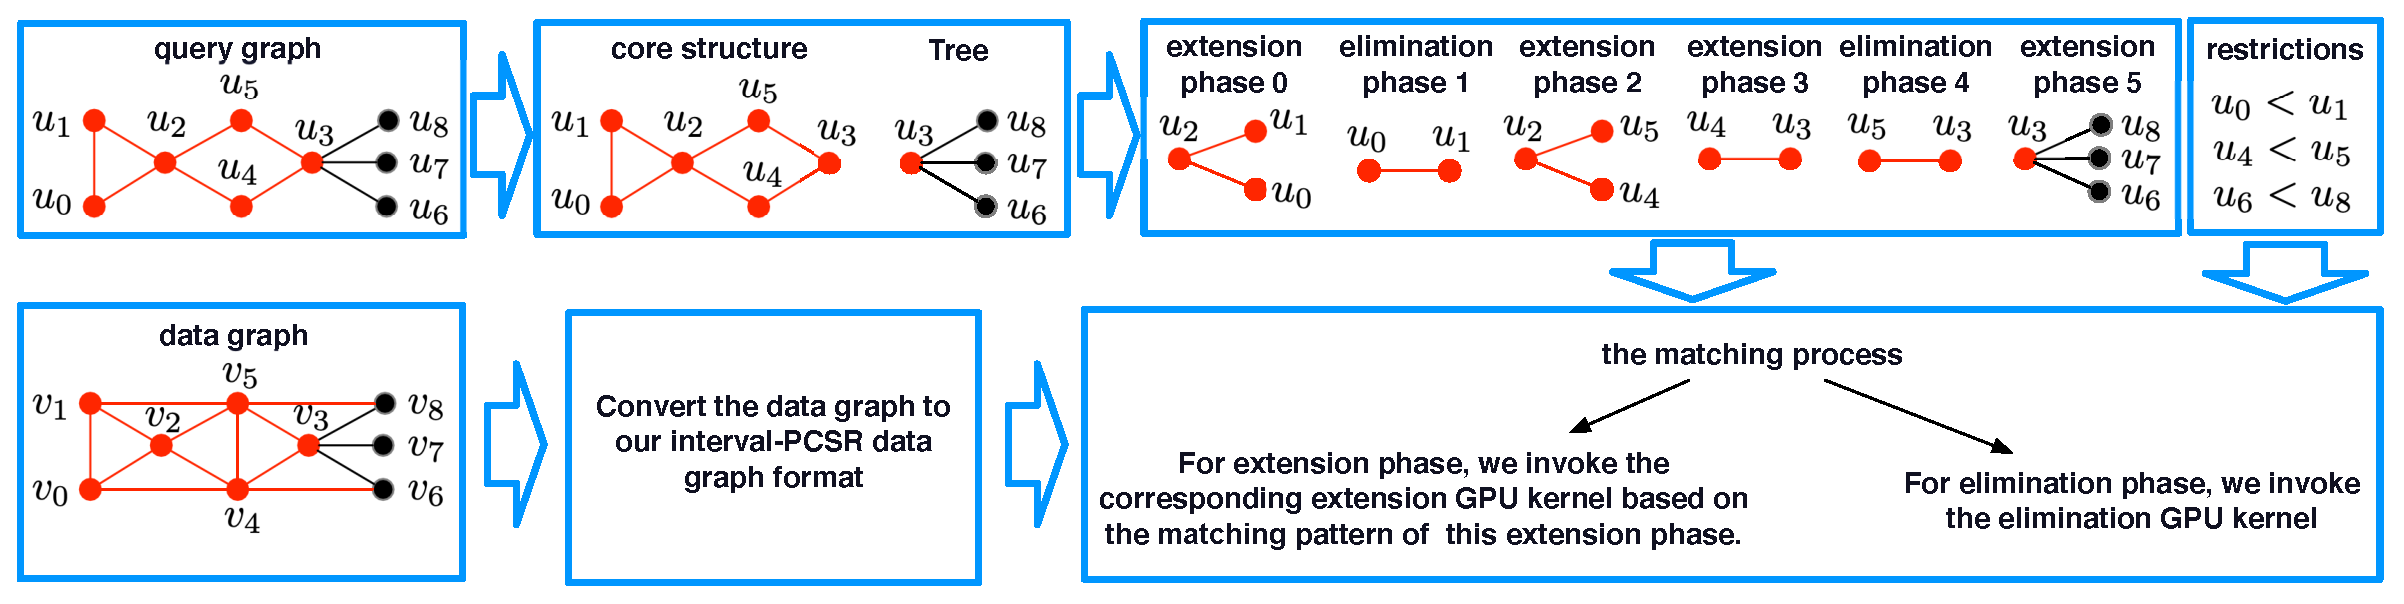
\includegraphics[width=\textwidth]{./figure/approachoverview.eps}
	\caption{An overview of our parallel vertex matching approach, \SystemName.}
	\label{fig:overview}
\end{figure*}

Figure~\ref{fig:overview} depicts the overall workflow of \SystemName. At the offline stage, we convert the data graph into a carefully
designed storage format. This format is designed to accelerate GPU kernel computation while reducing the GPU memory footprint when
processing large graphs (Section \ref{sec:storage}). We note that this storage conversion only needs to be performed once, which is a
one-off cost performed offline.

During runtime, \SystemName employs Algorithm \ref{algo:submatch} to perform subgraph search. This algorithm includes several steps. It
first decomposes the query graph into the core structure and trees according to the method proposed in \cite{bi2016efficient}. It then
further decomposse them into extension and elimination phases. Each extension phase contains exactly one matching pattern in Figure
\ref{fig:matchpattern} and each elimination phase contains one or more backward edges. In the meanwhile, it generates a matching order for
extension and elimination phases. It impose restrictions on query vertices (line 1) to avoid generating duplicate embeddings for symmetric
graphs (Section \ref{sec:pre}). All edges in an extension or elimination phase have the same edge label since we load one edge label
partition at each iteration (lines 2 and 7). The first extension phase of the matching order is used to generate the initial embeddings
(line 4). The main difference between the first and its following extension phases is that the source vertices of the former one are from
the edge label partition, while the later one are from previous embeddings. Finally, we use different GPU kernels to handle extension and
elimination phases (lines 10, 12), and output final embeddings (line 13). In the following sections, we elaborate each step in detail.

\section{Data Graph Storage Format\label{sec:storage}}
\begin{figure*}
\centering
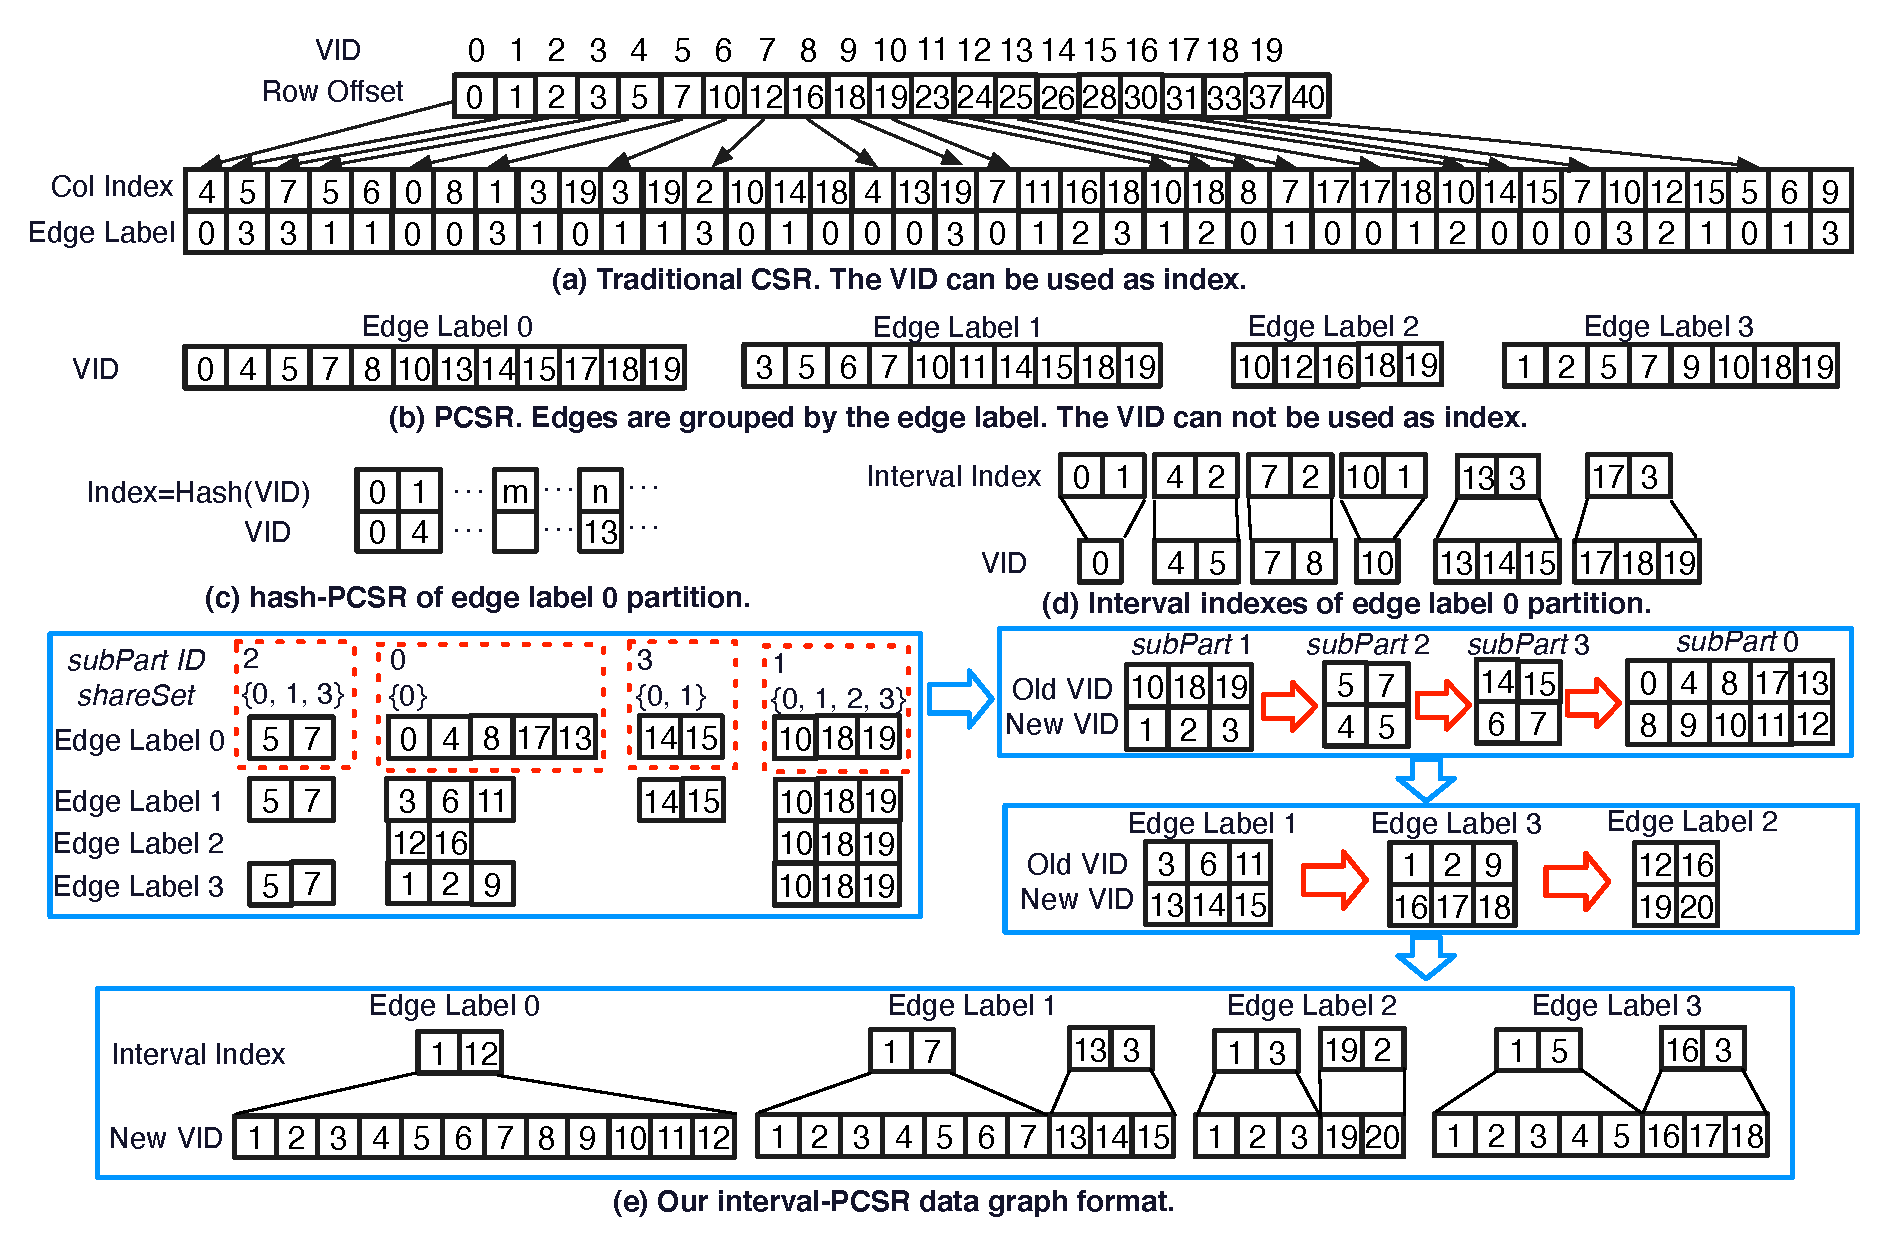
\includegraphics[width=\textwidth]{./figure/graphformat.eps}
\caption{Demonstration of data graph formats generated by traditional CSR (a), hash-PCSR that is used by GSI (b), non-optimized interval-PCSR (c), and our
optimized interval-PCSR (d). Note that VIDs in dashed squares do not need to be stored in memory.}	
\label{fig:dataformat}
\end{figure*}


\begin{algorithm}[t!]
\KwIn{the data graph in our format $G$, the query graph $q$} \KwOut{Embeddings of $q$ $EMB$} $\pi \leftarrow \textsc{GenMatchOrder}(q)$\;
Load the edge label partition $elp$ whose edge label is $\pi[0].edgeLabel$ from $G$ to GPU\; Allocate all available GPU memory space to
$newEMB$\; $\textsc{ExtKernel}(elp,NULL,newEMB,\pi[0])$\; $EMB \leftarrow newEMB$\; \For{$i \leftarrow 1$ \KwTo $\pi .size$}{
	Load the edge label partition $elp$ whose edge label is $\pi[i].edgeLabel$ from $G$ to GPU\;
	Allocate all available GPU memory space to $newEMB$\;
	\If{$\pi[i]$ is an extension phase}{
		$\textsc{ExtGPUKernel}(elp,EMB,newEMB,\pi[i])$\;
	}
	\Else{
		$\textsc{EliGPUKernel}(elp,EMB,newEMB,\pi[i])$\;
	}
	$EMB \leftarrow newEMB$\;
} \caption{\textsc{SubgraphSearch}} \label{algo:submatch}
\end{algorithm}

Real-world graphs are often too large to fit into the memory of a single GPU. Therefore, only part of the data that is needed for the
current computation should be stored in the GPU memory at a given time. As a result, it is important to find a compact representation of
the graph data without compromising the computation performance. To this end, \SystemName extends the Partitioned Compressed Sparse Row
(PCSR), the data graph storage format used by GSI \cite{zeng2020gsi}. This format groups edge with the same label into an edge label partition,
which is then stored in the Compressed Sparse Row (CSR) sparse matrix storage format. By doing so, only the partition with
the same edge label as the matching edge needs to be moved from the CPU memory into the GPU memory. PCSR makes some small modifications to
the CSR format. As depicted in Figure \ref{fig:dataformat}a, a vertex ID (VID) can be used to find the row offset of a vertex because VIDs are stored
as contiguous elements in a classical CSR. Because after grouping edges into partitions, VIDs of vertices are no longer guaranteed to be
continuous in the storage space, GSI employs a hash function to translate a VID into a slot the corresponding elements in the edge partition structure. To reduce collisions of the hash function, some empty entries have to be reserved
for each vertex (30 in GSI), which results in a large portion of unused GPU memory space. \SystemName is designed to avoid this pitfall.


\subsection{\SystemName Data Graph Storage Format}

\begin{algorithm}[t!]
\KwIn{the set of all edge label partitions $ELP$}
\KwOut{the mapping array $MAP$ with old and new VIDs are indices and values respectively}	
$newVID \leftarrow 1$\;
\While{ $ELP \neq \emptyset$ }{
	Choose the partition $elp \in ELP$ that has the most vertices\;
	Divide $elp$ into sub-partitions $subParts$\;
	\ForEach{$subPart \in subParts$}{
		Group IDs of partitions that contain $subPart$ into $shareSet$ and delete vertices of $subPart$ from these partitions\;
	}
	\While{$subParts \neq \emptyset$}{
		Choose the $subPart \in subParts$ that is shared by the most partitions and delete it from $subParts$\;
		Construct $MAP$ (assign new vertex IDs starting from $newVID$ to vertices in $subPart$ contiguously)\;
		$newVID \leftarrow newVID + subPart.size$\;
		$preSubPart \leftarrow subPart$\;
		\While{$preSubPart \neq \emptyset$}{
			Choose the $subPart \in subParts$ whose $shareSet$ has the most same partition IDs with the $shareSet$ of $preSubPart$ and delete the $subPart$ from $subParts$\;
			\If{Found the $subPart$}{
				Construct $MAP$\;
				$newVID \leftarrow newVID + subPart.size$\;
				$preSubPart \leftarrow subPart$\;
			}
			\Else{
				$preSubPart \leftarrow \emptyset$\;
				break\;
			}
		}
	}
	$ELP \leftarrow ELP/elp$\;
}
\caption{\textsc{GenMap}}
\label{algo:genmap}
\end{algorithm}

To reduce the amount of unused memory space required by the PCSR's hash function, we record the range of contiguous VIDs of an edge label
partition (ELP). The contiguous range of VIDs is recorded in an \emph{interval index} structure as shown in Figure \ref{fig:dataformat}c,
which stores the first VID and the number of continuous VIDs in the range.

Because an ELP may contain many small intervals, directly mapping each interval to be stored in an interval index will result in many
interval indices. This is not ideal because having a large number of interval indices means we will need many memory accesses to just find
the interval for a VID. For example, if we want to find the index of VID 7 in Figure \ref{fig:dataformat}c, with a naïve interval scheme,
we will have to compare number 7 against the first three interval indices before locating VID 7 in the third interval index. Our design
avoids this pitfall by carefully mapping the original VIDs to new VIDs, to allow one to generate more contiguous new VIDs in each edge
label partition, which in turn leads to a smaller number of intervals. Our data storage format shares the same spirit of Huffman coding \cite{Moffat2019Huffman} – we want to reduce the number of memory access when processing the largest ELP (i.e., the partition that contains the largest number of VIDs).

\subsection{\SystemName Storage Format Algorithm}

 As described in Algorithm \ref{algo:genmap} and Figure \ref{fig:dataformat}d, \SystemName takes several steps to convert the data graph into a GPU-tuned storage format, described as follows.

\cparagraph{Step 1: Find the largest ELP.} We start by choosing the partition that contains the most vertices (line 3 in Algorithm
\ref{algo:genmap}). Our intuition is that the more vertices a partition contains, the higher probability it will be accessed. Therefore,
reducing the number of intervals for this partition can help reduce the average memory access latency. For the example shown in Figure
\ref{fig:dataformat}d \textbf{\textcircled{1}}, edge label partition 0 is selected because it contains the largest number of vertices.

\cparagraph{Step 2: Rename VIDs.} In the second step, we try to increase the continuous VID interval by renaming the VIDs. To this end, for
each vertex, we find out all ELPs that contain the vertex. For example, vertices 4 and 8 in Figure \ref{fig:dataformat}d \textbf{\textcircled{1}} belong to ELPs 0,
1 and 2 - these ELPs form a share set for the two vertices. Next, we merge VIDs that have the same shares set into a subpartition (line 4
in Algorithm~\ref{algo:genmap}). For the example shown in Figure \ref{fig:dataformat}d \textbf{\textcircled{1}}, we map vertices 4 and 8 to a subpartition, subpart 0, because they have the same share set. We apply this grouping strategy to the largest ELP found in step 1. For the vertices that belong
to the same subpartition, we can assign unique, continuous new VIDs to them in arbitrary order, as long as these new VIDs are contiguous
and follow the largest VID from the last processed subpartition.

\cparagraph{Step 3: Process subpartitions.} To determine the order of the subpartitions of an ELP to be processed, we start from the
subpartition that is shared by most ELPs.  This means for the example shown in Figure \ref{fig:dataformat}d \textbf{\textcircled{1}}, we would first process
subpart 0, because it has the largest share set (with 3 ELPs).  The next subpartition we choose will be the one that has the largest number of common ELPs between its share set and the shared set of the last chosen subpartition. Looking at Figure \ref{fig:dataformat}d \textbf{\textcircled{1}} again, subpartition 1 will be the secondly chosen subpartition because its shared set has two ELPs ($0, 1$) with the share set of subpartition 0 (the firstly chosen subpartition). We choose this strategy because of the following two reasons.
First, the larger number of elements in common in the shared sets of two subpartitions, the more ELPs will have the two subpartitions.
Secondly, because we ensure the VIDs between two consecutively processed subpartitions are continuous, we can then merge the VIDs of the
two subpartitions to form a contiguous interval to be stored in a single interval index. Using this strategy, we can use a single interval index to record the new VIDs of subpartitions 0 and 1 in Figure \ref{fig:dataformat}d \textbf{\textcircled{2}}.


\cparagraph{Step 4: Repeat before Stop.} We delete the processed vertices from an ELP, and repeat steps 1 to 4 for each ELP in turn. This
process stops until all VIDs have been renamed and recored in the interval indices. This is illustrated in Figure \ref{fig:dataformat}d \textbf{\textcircled{3}}.


Figure \ref{fig:dataformat} shows the storage size of \SystemName against the PCSR scheme used by GSI for eight data graphs. The \SystemName storage
format reduces the storage size (and the GPU memory footprint) by 83\%.


\section{The Extension Phase\label{sec:extensionphase}}
Previous works \cite{zeng2020gsi,sun2020subgraph} adopt the traditional single vertex matching (SV-match) method when searching the query graph in a data graph. However, this method ignores some critical information of the query graph. The SV-match method needs to write intermediate results after matching a query vertex and read the same intermediate results before matching the next query vertex. This procedure is time-consuming because both write and read operations need to access GPU global memory. In order to speed up the matching process, we propose a parallel vertex matching method that can match as many vertices as possible in one step. Our method can handle all matching patterns shown in Figure \ref{fig:extpattern}.

The main problem of subgraph search on GPU is that the number of embeddings generated by each warp is different, thus we need to find the write address of newly generated embeddings for each warp to avoid write conflicts. To solve this problem, GSI \cite{zeng2020gsi} uses a Prealloc-Combine method, which needs two extra GPU kernels and access all embeddings twice to find the write address for each warp. Though Prealloc-Combine method is more efficient than GpSM \cite{tran2015fast} which generates embeddings twice, it still incurs high memory overhead. Different from GSI, we use $atomicAdd$ inside the GPU kernel to calculate write addresses. The main performance issue of $atomicAdd$ is the sequential execution when multiple warps update the same variable at the same time. But this is not a severe problem in subgraph matching because of the intrinsic irregularity of subgraph matching.


Algorithm \ref{algo:extphase} describes the overall workflow of the extension phase. For each embedding (line 3), we first obtain source VIDs from the embedding according to the matching pattern that the extension phase contains (line 4). Then, we search source VIDs in the interval-PCSR of the loaded edge label partition, and extract their neighbors (line 5).  Next, we remove invalid neighbors that have wrong vertex labels and do not satisfy restrictions. Finally, we use different algorithms to generate new embeddings for different matching patterns (lines 8-15). In the following of this section, we first describe embedding generation methods for matching patterns 2-4, then an optimized generation method for the matching pattern 1, and finally generation methods of matching patterns 5-7 that are based on extension pattern 1.

\begin{algorithm}
\KwIn{the edge label partition $elp$, partial embeddings $EMB$, the starting address of new embeddings $newEMB$, the extension phase $extP$}
$totNum \leftarrow 0$\;
Load interval indexes of $elp$ into shared memory\;
\ForEach{$emb \in EMB$}{
	Get source VIDs $u_{s1}$ and $u_{s2}$ from $emb$\;
	Search $u_{s1}$ and $u_{s2}$ in interval indexes and extract their neighbors $ne1$ and $ne2$, respectively.\;
	Remove neighbors that do not have the same vertex labels as $u_{1}$ and $u_{2}$ from $ne1$ and $ne2$, respectively\;
	Remove neighbors that do not satisfy the restrictions of $u_{1}$ and $u_{2}$ from $ne1$ and $ne2$, respectively\;
	\If{$extP$ is matching pattern 0}{
		We use the traditional SV-ext method to generate embeddings for $extP$\;
	}
	\ElseIf{$extP$ is matching pattern 1}{
		$\textsc{OptDouExt}(emb,ne1,totNum,newEMB)$\;
	}
	\ElseIf{$extP$ is one of matching patterns 2, 3, and 4}{
		$\textsc{DouExt}(emb,ne1,ne2,totNum,newEMB)$\;
	}
	\ElseIf{$extP$ is one of matching patterns 5, 6, and 7}{
		$\textsc{NExt}(emb,ne1,ne2,totNum,newEMB,extP)$\;
	}
}

\caption{\textsc{ExtPhaseKernel}}
\label{algo:extphase}
\end{algorithm}

For matching patterns 2-4, we devise a direct method, Algorithm \ref{algo:generalDV}, to generate new embeddings. The main idea of Algorithm \ref{algo:generalDV} is to iterate over all combinations of candidates of $u_{1}$ and $u_{2}$, denoted as $C_1$ and $C_2$ respectively, and construct new embeddings by appending each valid combination to a new copy of the current embedding $emb$. We say a combination is valid, if neither VIDs in the combination equal to VIDs in $emb$. To avoid checking this condition repeatedly, we first check this condition for all vertices in $C_2$ once (lines 3-4) and record indexes of vertices whose VIDs also exist in $emb$ (line 5). To fully utilize $C_2$, we generate new embeddings while checking the condition. Once a vertex in $C_2$ is checked valid (lines 6-7), we assign this vertex and the first valid vertex in $C_1$ to $u_2$ and $u_1$, respectively (lines 1,8). Then, we write the new embedding $(emb,u_1,u_2)$ to the corresponding address (lines 9-10).

\begin{algorithm}
	\KwIn{the partial embedding $emb$, candidates of $u_1$ $C_1$, candidates of $u_2$ $C_2$, the number of newly written embeddings $totNum$, the starting address of new embeddings $newEMB$}
	Find the index $i$ of the first valid vertex in $ne1$\;
	$writePos \leftarrow atomicAdd(totNum,1 \times C_{2}.size)$\;
	\For{$j \leftarrow 0$ \KwTo $C_{2}.size$}{
		\If{$C_2[j] \in emb$}{
			Add $j$ to the set $boundry$\;
			$u_1 \leftarrow 0$; $u_2 \leftarrow 0$\;
		}
		\Else{
			$u_1 \leftarrow C_1[i]$; $u_2 \leftarrow C_2[j]$\;
		}
		Write the new embedding ($emb$, $u_1$, $u_2$) to the address pointed by $newEMB+writePos$\;
		$writePos \leftarrow writePos + emb.size+2$\;
	}
	$i \leftarrow i+1$\;
	\While{$i < C_{1}.size$}{
		Load 32 candidates from $C_1$ into $tmp$; $i \leftarrow i+32$\;
		Remove candidates that exist in $emb$ from $tmp$\;
		$writePos \leftarrow atomicAdd(totNum,tmp.size \times (C_{2}.size-boundry.size))$\;
		\ForEach{$0 \leq k<tmp.size$ and $0 \leq j<C_{2}.size$ and $j \notin boundry$}{
			\If{This is EP 2 and $C_1[k]=C_2[j]$}{
				$u_1 \leftarrow 0$; $u_2 \leftarrow 0$\;
			}
			\Else{
				$u_1 \leftarrow C_1[k]$; $u_2 \leftarrow C_2[j]$\;
			}
			Write the new embedding ($emb$, $u_1$, $u_2$) to the address pointed by $newEMB+writePos$\;
			$writePos \leftarrow writePos + emb.size+2$\;
		}
	}
	\caption{\textsc{DouExt}}
	\label{algo:generalDV}
\end{algorithm}

At the beginning of Algorithm \ref{algo:generalDV}, we allocate space for new embeddings generated when checking conditions for $C_2$ (line 2). Since we do not know the number of valid vertices in $C_2$ until all vertices are checked, we use the vertex count of $C_2$, denoted as $C_{2}.size$, to overestimate the number of new embeddings. If there are invalid vertices in $C_2$, we assign 0 to $u_1$ and $u_2$ to indicate invalid embeddings (line 6). When a GPU kernel read an embedding that contains 0, it skips processing it.

In Algorithm \ref{algo:generalDV}, after finding invalid vertices in $C_2$, we generate new embeddings for rest vertices in $C_1$ (lines 11-12). In each iteration, we load 32 vertices in $C_1$ into shared memory $tmp$ and remove invalid ones from $tmp$ (lines 13-14). In order to allocate space for new embeddings, we estimate its count as the number of combinations of $tmp$ and valid vertices in $C_2$ (line 15). Then, we generate new embeddings for these combinations (line 16). As $u_1$ and $u_2$ have the same vertex label in extension pattern 2, there is a chance that two candidates of $u_1$ and $u_2$ are equal (line 17), which makes the generated new embedding invalid. To solve the problem, we assign 0 to $u_1$ and $u_2$ if the embedding is invalid (line 18), otherwise assign corresponding candidates to $u_1$ and $u_2$ (line 20). Finally, write the new embedding to the specified address (lines 21-22).

However, Algorithm \ref{algo:generalDV} is not appropriate for the matching pattern 1. In the matching pattern 1, $u_1$ and $u_2$ are extended from the same source vertex $u_{s1}$ and have the same vertex label, thus $C_1 = C_2$. If Algorithm \ref{algo:generalDV} is applied to the matching pattern 1, each vertex in $C_2$ can be accessed by up to $C_1.size$ times. As shown in the left part of Figure \ref{fig:ep1opt}, element 1 is accessed at each iteration of $i$. If $C_1.size>32$, we need to reload element 1 from global memory each time we access it. Other elements also encounter the same problem.

\begin{figure}
\centering
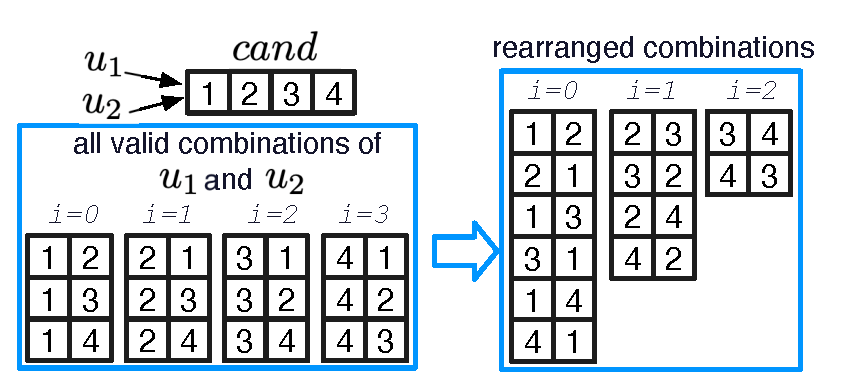
\includegraphics[width=\columnwidth]{./figure/ep1opt.eps}
\caption{An example of generating new embeddings for the matching pattern 1.}	
\label{fig:ep1opt}
\end{figure}

To speed up the matching process of the matching pattern 1, we rearrange the generation order of combinations, as shown in the right part of Figure \ref{fig:ep1opt}, to make accesses more register friendly. Algorithm \ref{algo:optDV} demonstrates the core design of the optimized generation method for the matching pattern 1. From the right part of Figure \ref{fig:ep1opt}, we make two important observations to guide the design of Algorithm \ref{algo:optDV}. First, the element $C_1[i]$ is only used at iteration $i$ and thus we load it into a register (line 2) to reduce its access latency. Second, each time we generate a combination, we can reverse the combination to obtain another combination immediately without reloading data from global memory (lines 4-5).

\begin{algorithm}
	\KwIn{embeddings $emb$, candidates $C$, the number of newly written embeddings $totNum$, the starting address of new embeddings $newEMB$}
	$writePos \leftarrow atomicAdd(totNum,C.size \times (C.size-1))$\;
	\For{$i \leftarrow 0$ \KwTo $C.size-1$}{
		\For{$j \leftarrow i+1$ \KwTo $C.size$}{
			Write new embeddings ($emb$, $C[i]$, $C[j]$) and ($emb$, $C[j]$, $C[i]$) to the address pointed by $newEMB+writePos$\;
			$writePos \leftarrow writePos + (emb.size+2) \times 2$\;
		}
	}
	\caption{\textsc{OptDouExt}}
	\label{algo:optDV}
\end{algorithm}

\begin{algorithm}
	\KwIn{embeddings $emb$, candidates of \{$u_1, \cdots, u_n$\} $C_1$, candidates of \{$u_{n+1}, \cdots, u_{n+m}$\} $C_2$, the number of newly written embeddings $totNum$, the starting address of new embeddings $newEMB$, extension phase $extP$}
	\If{$extP$ is matching pattern 5}{
		\ForEach{$comb1$ of combinations of $u_1, \cdots, u_{n-2}$}{
			$emb_{copy} \leftarrow (emb, comb1)$; $C_{copy} \leftarrow C_1/comb1$\;
			$\textsc{OptDouExt}(emb_{copy},C_{copy},totNum,newEMB)$\;
		}
	}
	\ElseIf{$extP$ is one of matching patterns 6 and 7}{
		\ForEach{$comb2$ of combinations of $u_{n+1}, \cdots, u_{n+m}$}{
			\ForEach{$comb1$ of combinations of $u_1, \cdots, u_{n-2}$}{
				$emb_{copy} \leftarrow (emb, comb1, comb2)$; $C_{copy} \leftarrow C_1/comb1$\;
				$\textsc{OptDouExt}(emb_{copy},C_{copy},totNum,newEMB)$\;
			}
		}
	}
	\caption{\textsc{NExt}}
	\label{algo:nvext}
\end{algorithm}

We design Algorithm \ref{algo:nvext} to generate embeddings for matching patterns 5-7 based on Algorithm \ref{algo:optDV}. For the matching pattern 5 (line 1), we iterate over all combinations of $u_1, \cdots, u_{n-2}$ (line 2) and use Algorithm \ref{algo:optDV} to match last two query vertices $u_{n-1}$ and $u_n$ (line 4). Before invoking Algorithm \ref{algo:optDV}, we need to construct a new embedding and new candidates for $u_{n-1}$ and $u_n$ (line 3). For matching patterns 6 and 7, we first use an outer loop to iterate over all combinations of $u_{n+1}, \cdots, u_{n+m}$, and use the same method as the matching pattern 5 to generate embeddings (lines 7-9).

When decomposing the query graph into extension and elimination phases, there is a possibility that multiple matching patterns are available for an extension phase. To choose the most suitable matching pattern, we assign 2-level priorities to matching patterns. In the first level, we prioritize matching patterns based on the number of query vertices to be matched in each matching pattern. Thus, matching patterns 5-7 get the highest priority, 1-4 get the medium priority, and 0 gets the lowest priority. In the second level, we prioritize matching patterns that posses the same first level priority based on efficiency of each matching pattern when generating embeddings.

We first analyze the efficiency of medium priority matching patterns, and then the highest priority ones. The matching pattern 1 uses an optimized method (Algorithm \ref{algo:optDV}) to generate embeddings, thus it is most efficient among matching patterns 1-4. matching patterns 2-4 use the normal method (Algorithm \ref{algo:generalDV}) but the matching pattern 2 needs to evaluate the equality of candidates of $u_1$ and $u_2$. Therefore, the matching pattern 2 is the least efficient one. Compared to the matching pattern 3, the matching pattern 4 needs one more step to find the address of $u_{s2}$, thus it is less efficient than the matching pattern 3. Consequently, the priority order of matching patterns 1-4 from the highest to the lowest is matching pattern 1, 3, 4, and 2.

Among matching patterns of the highest priority, the matching pattern 5 is the most efficient one because it only needs one step to find the neighbor address of $u_{s1}$ in the edge label partition and another step to find the address of neighbors that have the same vertex label as $u_1, \cdots, u_n$. In contrast, the matching pattern 7 is the least efficient one because it needs one more step to find the neighbor address of $u_{s2}$ compared to the matching pattern 5. Consequently, the priority order of matching patterns 5-7 from the highest to the lowest is matching pattern 5, 6, and 7.

\section{The Elimination Phase\label{sec:eliphase}}
GSI \cite{zeng2020gsi} matches only one query edge in a GPU kernel and Lai et al. \cite{lai2015scalable} matches at most two query edges at each iteration. Both methods can not fully utilize the elimination power of backward edges. In our approach, we match as many backward edges as possible to eliminate invalid embeddings at early stages. Algorithm \ref{algo:eliphase} demonstrates how our approach deals with the eliminate phase. For each embedding $emb$ (line 2), we first check if all query edges in the elimination phase can be matched in $emb$ (line 4). If so (line 5), we write $emb$ to the shared memory $tmp$ (line 6) and write $tmp$ to global memory if it is full (lines 7-9).


\begin{algorithm}
\KwIn{the edge label partition $elp$, embeddings $EMB$, the number of generted embeddings $totNum$, the elimination phase $eliPhase$}
Load interval indexes of $elp$ into shared memory\;
\ForEach{$emb \in EMB$}{
	\ForEach{$edge \in eliPhase$}{
		Check if there is an edge in $emb$ that can match $edge$\;
	}
	\If{all edges in $eliPhase$ are matched}{
		Write $emb$ to shared memory $tmp$\;
		\If{$tmp$ is full}{
			$writePos \leftarrow atomicAdd(totNum,tmp.size)$\;
			Write $tmp$ to the address pointed by $newEMB+writePos$\;
		}
	}
}
\caption{\textsc{EliPhaseKernel}}
\label{algo:eliphase}
\end{algorithm}




\section{Matching Order\label{sec:matchingorder}}

In this section, we first give a brief description of matching order generation method used in \cite{bi2016efficient}, and then demonstrate the details of our matching order generation algorithm based on parallel vertex matching method.

The main goal of \cite{bi2016efficient} is to match backward edges as soon as possible to eliminate invalid embeddings at early stages. Therefore, they generate a subgraph of $q$ that contains all backward edges regarding any spanning tree of $q$ by iteratively removing all degree-one vertices from $q$. The generated subgraph, which is called the core structure as shown in Figure \ref{fig:overview}, is matched first. In our approach, we also match the core structure first, and then the trees.

When decomposing the core structure into extension and elimination phases, we need to adhere to an important constraint, which is that only matching patterns 0-4 can be used to decompose the core structure. The reason is explained as follows. In order to eliminate invalid embeddings as soon as possible, we need to first match circles in the core structure, which are $\{u_0, u_1, u_2\}$ and $\{u_2, u_3, u_4, u_5\}$ in Figure \ref{fig:overview}. Therefore, we only need to match at most two vertices when matching a circle because vertices in a circle have exactly two neighbors. Figure \ref{fig:overview} demonstrates that the core structure is decomposed with matching patterns 0-4. We can see in the core structure that $u_0$, $u_1$, $u_2$, $u_4$, and $u_5$ can be matched with the matching pattern 5 where $u_2$ is the source vertex. If we first decompose the core structure with the matching pattern 5, and then the backward edge $(u_0, u_1)$, a large number of invalid embeddings may be generated before matching the backward edge $(u_0, u_1)$, which significantly slows down the matching performance. After matching the core structure, we can use any appropriate matching patters to match trees. For example, the matching pattern 5 can be used to match the tree in Figure \ref{fig:overview}.


Based on \cite{bi2016efficient} and our parallel vertex matching method, we design Algorithm \ref{algo:genmatchorder} to generate matching order of extension and elimination phases. At the beginning of Algorithm \ref{algo:genmatchorder}, we adopt methods proposed in \cite{shi2020graphpi,mawhirter2019graphzero} to generate restrictions on VIDs in embeddings (line 1). Thus, we can avoid generating automorphic embeddings. Then we generate the core structure of $q$ by iteratively removing degree-one vertices from $q$, and construct trees of $q$ using removed vertices (line 2).

In order to match the core structure, we first find the smallest circle in the core structure (line 3), and then select vertices in the circle that conform to the highest priority matching pattern among matching patterns 0, 1, and 3 (line 4). The selected vertices constitute the initial phase (lines 5-6), which is a special kind of extension phase. Different from the normal extension phase that fetches source vertices from embeddings, the initial phase fetches the source vertex from the edge label partition. After generating the initial phase, we iteratively find vertices in the circle that conform to matching patterns 0-4 and choose the one with the highest priority (lines 7-9). Finally, we use the backward edge in the circle to construct an elimination phase (line 10).

After decomposing the smallest circle, we iteratively construct extension and elimination phases for the rest vertices and edges in the core structure (line 11). First, we find all backward edges and group them by the edge label (lines 12-13). For each group, we construct an elimination phase (lines 14-15). If no backward edges are found, we search for unmatched vertices in the core structure that can form one of matching patterns 0-4, and choose the one with the highest priority (lines 16-18).

After matching the core structure, we can use any appropriate matching patterns in Figure~\ref{fig:matchpattern} to match rest vertices that are not in the core structure since there is no backward edge left. At each iteration, we find vertices that can form matching patterns 0-7 and select the one with the highest priority (lines 19-21).


\begin{algorithm}
	\KwIn{the query graph $q$}
	\KwOut{the match phase queue $matchPhase$}
	Generate restrictions to eliminate automorphisms\;
	Generate the core structure $C$ and trees $T$ of $q$\;
	Find the smallest circle $minc$ in $C$\;
	Select vertices in $minc$ that conform to matching patterns 0, 1, and 3, and choose the highest priority matching pattern\;
	Construct the initial phase with vertices corresponding to the selected matching pattern\;
	Add the initial phase to $matchPhase$\;
	\For{vertices in $minc$ that conform to matching patterns 0-4}{
		Choose the highest priority matching pattern and construct an extension phase\;
		Add the extension phase to $matchPhase$\;
	}
	Construct an elimination phase with the backward edge in $minc$ and add it to $matchPhase$\;
	\For{rest vertices and edges in $C$}{
		\If{there are backward edges}{
			Group all backward edges by the edge label\;
			\ForEach{group $g$}{
				Construct an elimination phase $eliPhase$ based on $g$ and add it to $matchPhase$\;
			}	
		}
		\Else{
			Find vertices that conform to matching patterns 0-4 and choose the one with the highest priority\;
			Construct an extension phase and add it to $matchPhase$\;
		}
	}
	\For{vertices in $T$}{
		Find vertices that can form matching patterns 0-7 and select the one with the highest priority\;
		Construct an extension phase and add it to $matchPhase$\;
	}
	\caption{\textsc{GenMatchOrder}}
	\label{algo:genmatchorder}
\end{algorithm}


\section{Load Balance} In GPU, once a thread block is scheduled to run on an SM, it will not be scheduled out until all warps in this
thread block are finished. Therefore, if one warp matches a vertex or an edge that has many candidates, all warps in the same thread block
have to wait for its completion. To address this problem, GSI designs a four-layer balance scheme. However, their scheme needs to invoke a
GPU kernel inside a GPU kernel, which is time-consuming as illustrated in Section \ref{sec:compargsi}. Different from GSI, we use fixed
warps, which means that the maximum concurrent warps are generated and will not be scheduled out during execution, to perform subgraph search.
In this way, a warp with small workload can match next embedding without waiting for other warps. Only when there is no embeddings left,
the faster warps have to wait for the slower warps. Our approach is simple yet effective, it can mitigate load imbalance to some extend. A
more powerful load balance scheme can be designed and we leave this for a future study.
